\subsection{Solucion desarrollada}

\begin{trampa}{Consistencia de datos}
Aqui no hay una inconsistencia conceptual, sino una inconsistencia numerica entre las fuentes del ejercicio. La tabla de 27 pesos suma correctamente
\[
\sum_{i=1}^{27}x_i=9538,
\]
lo que coincide con el enunciado. Sin embargo, al elevar esos mismos datos al cuadrado se obtiene:
\[
\begin{array}{c|rrrrrrrrr}
i & 1&2&3&4&5&6&7&8&9\\
\hline
x_i^2 & 116964&126736&145161&103684&126025&128881&135424&116281&110889
\end{array}
\]
\[
\begin{array}{c|rrrrrrrrr}
i & 10&11&12&13&14&15&16&17&18\\
\hline
x_i^2 & 116964&133956&137641&115600&136900&133225&125316&124609&106276
\end{array}
\]
\[
\begin{array}{c|rrrrrrrrr}
i & 19&20&21&22&23&24&25&26&27\\
\hline
x_i^2 & 141376&102400&128881&142884&157609&101761&120409&139876&104976
\end{array}
\]
Por lo tanto, desde la tabla:
\[
\sum_{i=1}^{27}x_i^2=3380704,
\]
mientras que el enunciado impreso declara
\[
\sum_{i=1}^{27}x_i^2=3376759.
\]
La diferencia es:
\[
3380704-3376759=3945.
\]
Ademas, la pauta manuscrita parece trabajar con \(\sigma\approx 15.6\), que tampoco sale exactamente ni de la tabla ni del agregado impreso. Por eso hay tres caminos numericos posibles: respetar la tabla, respetar los agregados impresos, o seguir la pauta manuscrita. En esta solucion se usa como criterio principal el agregado impreso del enunciado, porque es el dato resumido que el problema entrega explicitamente para calcular la desviacion estandar. La pauta manuscrita queda como referencia alternativa.
\end{trampa}

\begin{respuesta}{(a) Media y desviacion estandar}
La media muestral se calcula como:
\[
\bar x=\frac{\sum_{i=1}^{27}x_i}{27}
=\frac{9538}{27}=353.26\ \text{g}.
\]

Usando el agregado impreso \(\sum x_i^2=3376759\), la desviacion estandar del proceso se calcula como:
\[
\sigma
=\sqrt{\frac{3376759}{27}-353.26^2}
=16.52\ \text{g}.
\]
Por lo tanto:
\[
\boxed{\bar x=353.26\ \text{g}},\qquad
\boxed{\sigma=16.52\ \text{g}}.
\]

Si se usara la tabla completa, entonces:
\[
\sigma_{\text{tabla}}
=\sqrt{\frac{3380704}{27}-353.26^2}
=20.47\ \text{g}.
\]
Esta diferencia explica por que el diagnostico puede cambiar segun la fuente numerica que se decida respetar.
\end{respuesta}

\begin{respuesta}{(b) Limites de control al 96\%}
Para un nivel de confianza de \(96\%\), se usa:
\[
z=2.055.
\]
Reemplazando \(\bar x=353.26\), \(\sigma=16.52\) y \(z=2.055\):
\[
LCI=\bar x-z\sigma
=353.26-2.055(16.52)=319.30\ \text{g},
\]
\[
LCS=\bar x+z\sigma
=353.26+2.055(16.52)=387.22\ \text{g}.
\]
Por lo tanto:
\[
\boxed{LCI=319.30\ \text{g}},\qquad
\boxed{LC=353.26\ \text{g}},\qquad
\boxed{LCS=387.22\ \text{g}}.
\]
\end{respuesta}

\begin{respuesta}{(c) Grafico con los limites de control}
El grafico inicial se construye poniendo en el eje horizontal el numero de muestra y en el eje vertical el peso observado. La linea central corresponde a \(\bar x=353.26\), y las lineas punteadas a \(LCI=319.30\) y \(LCS=387.22\).

\begin{center}
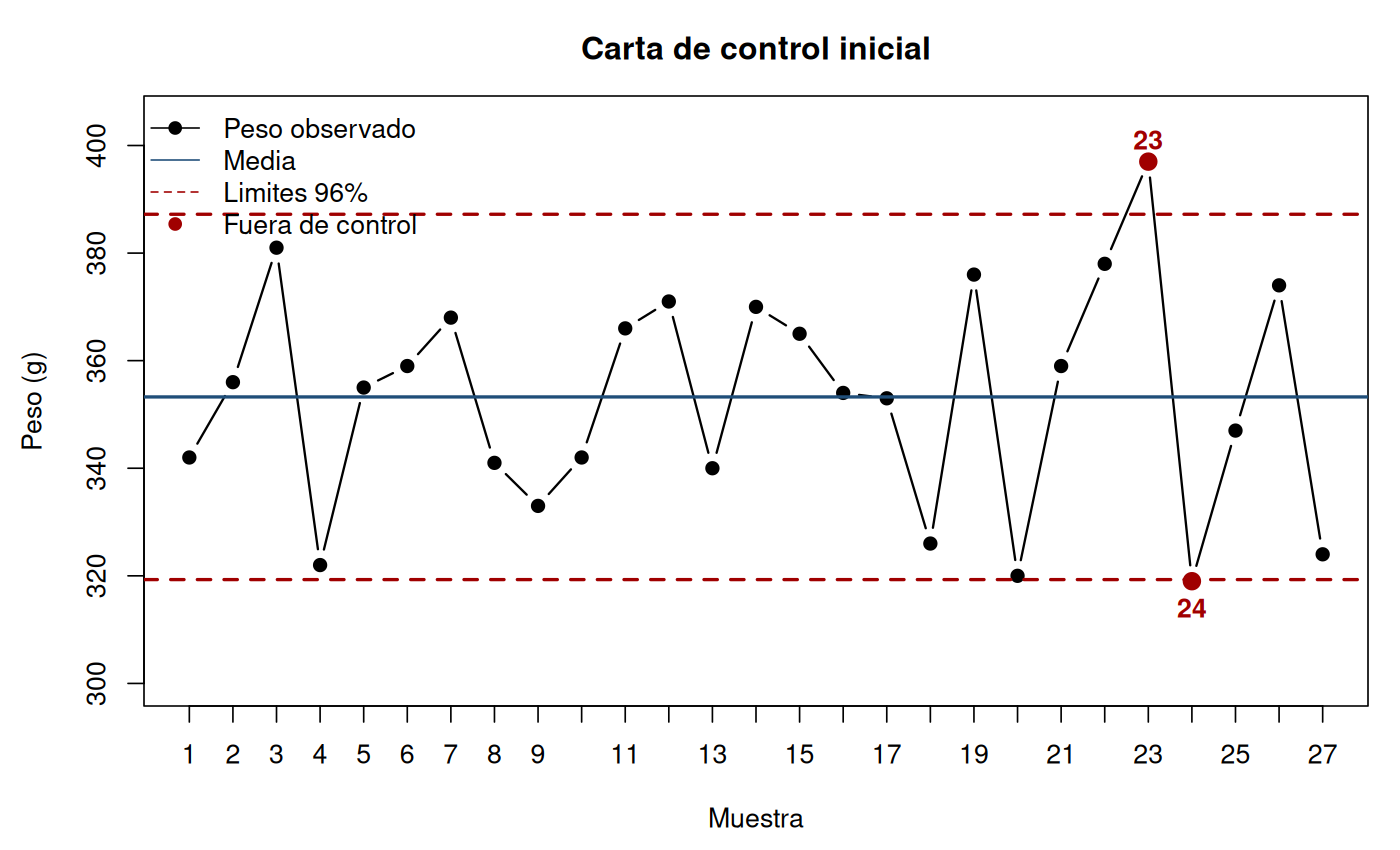
\includegraphics[width=0.92\textwidth]{ejercicios/02/figuras/control_inicial.png}
\end{center}
\end{respuesta}

\begin{respuesta}{(d) Diagnostico del proceso y recalculo}
El proceso no se encuentra bajo control, porque existen observaciones fuera de los limites:
\[
x_{23}=397>387.22,
\qquad
x_{24}=319<319.30.
\]
Por lo tanto:
\[
\boxed{\text{muestras fuera de control: }23,\ 24.}
\]

Al eliminar esas observaciones por causa asignable, quedan \(25\) datos. Manteniendo el mismo criterio de usar los agregados impresos, la nueva media es:
\[
\bar x_{\text{nuevo}}
=\frac{9538-397-319}{25}
=352.88\ \text{g}.
\]
La nueva desviacion estandar se calcula restando del agregado impreso los cuadrados de las observaciones eliminadas:
\[
\sigma_{\text{nuevo}}
=\sqrt{
\frac{3376759-397^2-319^2}{25}
-352.88^2
}
=13.09\ \text{g}.
\]
Luego:
\[
LCI_{\text{nuevo}}
=352.88-2.055(13.09)
=325.99\ \text{g},
\]
\[
LCS_{\text{nuevo}}
=352.88+2.055(13.09)
=379.77\ \text{g}.
\]

El grafico recalculado queda:

\begin{center}
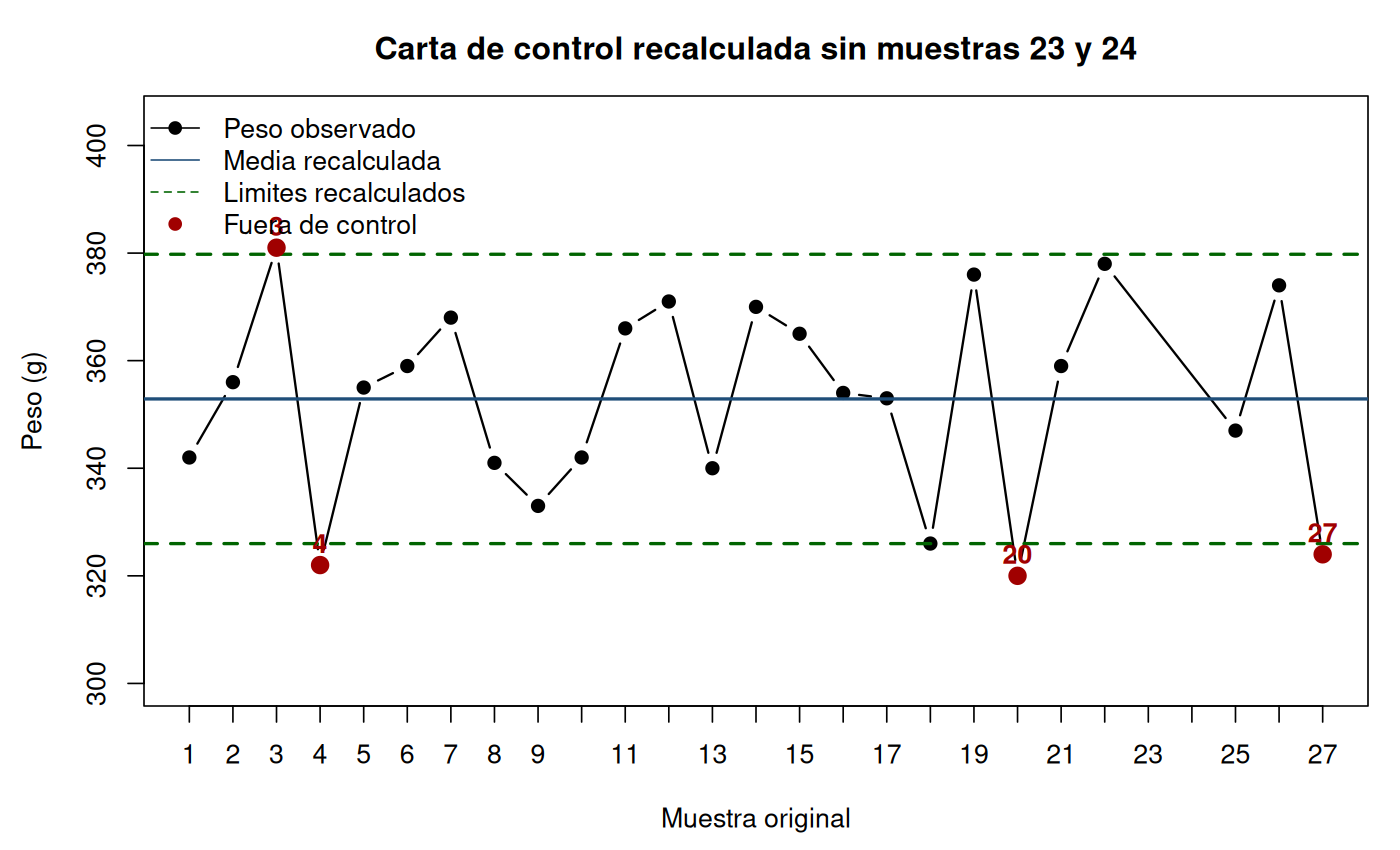
\includegraphics[width=0.92\textwidth]{ejercicios/02/figuras/control_recalculado.png}
\end{center}

Con estos nuevos limites, aparece una nueva observacion fuera de control:
\[
x_3=381>379.77.
\]
Por lo tanto, bajo el criterio de agregados impresos, al retirar las muestras \(23\) y \(24\) el proceso todavia no queda completamente bajo control; el grafico recalculado muestra que la muestra \(3\) tambien debe investigarse como posible causa asignable.
\end{respuesta}

\begin{trampa}{Que escribir si corriges con la pauta manuscrita}
Si el corrector exige seguir la pauta manuscrita, entonces se usa \(\sigma\approx 15.6\), \(LCI=321.20\), \(LCS=385.40\), y las muestras fuera de control son \(20\), \(23\) y \(24\). Si se calcula todo desde la tabla, entonces \(\sigma=20.47\), \(LCI=311.19\), \(LCS=395.33\), y solo queda fuera la muestra \(23\). En una prueba, conviene declarar claramente que se estan usando los agregados impresos del enunciado; bajo ese criterio, \(\sigma=16.52\).
\end{trampa}
